\chapter{提案手法の検証実験}
%\section{信号検出性能}
%距離、ダイレクトパスなしなどの状況を変えて

\section{同期手法の有効性}

本手法における端末間距離測定を評価した.MacBookPro13 インチ 4 台を,図\ref{fig:relpos}に配置し,先述 のアルゴリズムにより各端末間距離を 50 回計測した結果を表\ref{tab:estdistance}に示す.
計測された各端末間の信号伝達時間と音速 を 340m/s と仮定したときの計測距離より,誤差は平均で30cm程度となりDBAP法での音源生成には問題が生じない程度の精度を得られた.
また,距離計測性能と同期性能は比例するため,距離が正しく測定されていれば同期性能も十分であると言える.

\begin{figure}[p]
  \begin{center}
    \begin{tabular}{c}
      \begin{minipage}{0.3\hsize}
        \begin{center}
          \hspace{-2mm}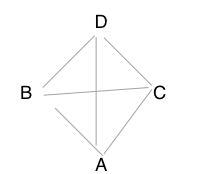
\includegraphics[clip,width=1\hsize]{img/PC_haichi.png}
          \caption{PC配置}
          \label{fig:relpos}
        \end{center}
      \end{minipage}
      \begin{minipage}{0.68\hsize}
        \begin{center}
          \caption{50回試行時の端末間距離計測結果}
          \begin{tabular}{l|rrrrr}
            \hline
            {\footnotesize  端末間}&{\footnotesize 平均}&{\footnotesize 標準偏差}&{\footnotesize 実測距離(m) }\\
            \hline
            {\footnotesize A-D }&{\footnotesize 11.71889953}&{\footnotesize 1.24793883}&{\footnotesize 11.10 }\\
            {\footnotesize B-D }&{\footnotesize 7.767573696}&{\footnotesize 0.583510141}&{\footnotesize 7.77 }\\
            {\footnotesize C-D }&{\footnotesize 6.72675737}&{\footnotesize 0.774180135}&{\footnotesize 6.72 }\\
            {\footnotesize A-B }&{\footnotesize 6.564537924}&{\footnotesize 1.067679838}&{\footnotesize 6.83 }\\
            {\footnotesize A-C }&{\footnotesize 7.300425749}&{\footnotesize 1.283308926}&{\footnotesize 6.93 }\\
            {\footnotesize B-C }&{\footnotesize 4.771470221}&{\footnotesize 0.664454607}&{\footnotesize 4.92 }\\
            \hline
          \end{tabular}
          \label{tab:estdistance}
        \end{center}
      \end{minipage}
    \end{tabular}
  \end{center}
\end{figure}



\section{DBAP法の有効性}

被験者の聴衆実験を行った.
被験者の向きの要因-45,0,45,90度,
距離要因として端末群の端から-1.15,0,1,2.31,4.62m,
音源位置を4箇所に用意し,音源位置を答えさせた.
実験結果を図\ref{fig:gosa},\ref{fig:hikenshaichi},\ref{fig:ongenichi}に示す.
距離が遠いと誤差があるものの,誤差は1メートル前後である.
端末数が少ない(4台)でDBAPをしてアレイの外にいる受聴者が音像を4台の中に感じたのは当然の結果である.
内部に入るとまったく定位できなくなった.
教室内で利用するときに,100人規模,20-30m平米の教室であれば,この程度の誤差は許容できる.


DBAP法の原理上,音のみかけの幅(ASW)と,音に包まれた感じ(LEW)が生じる\cite{ku-kanonkyo, onbasaigen, onkyoukougaku, 森本政之, 森本政之09, 森本政之90, 森本政之93, 崔瑛芝, 上杉信敏, 田中雅史}
もっと高密度に端末が分布している時のDBAPの効果が知りたい


\begin{figure}[p]
  \centering
  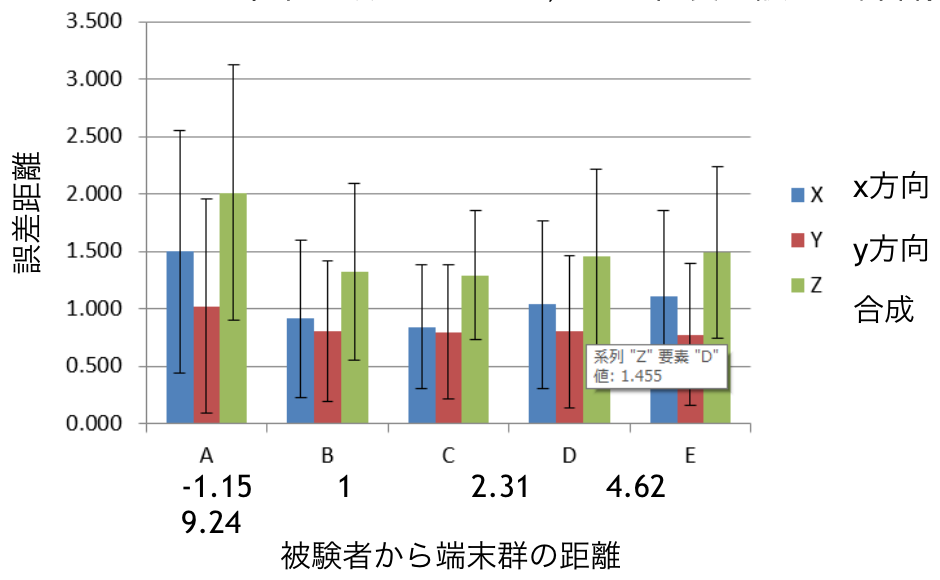
\includegraphics[clip,width=1.05\hsize]{img/bougurahu.png}
  \caption{誤差距離}\label{fig:gosa}
\end{figure}


\begin{figure}[p]
  \centering
  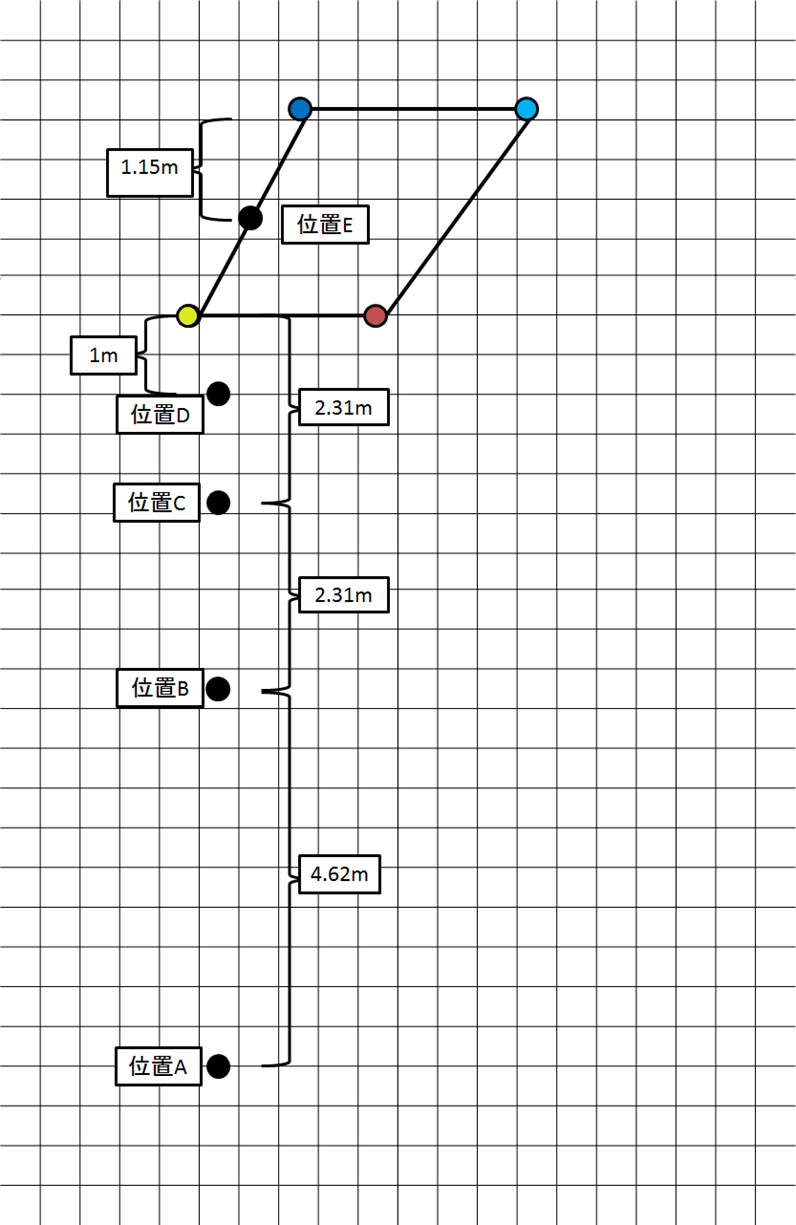
\includegraphics[clip,width=1.05\hsize]{img/hikenshaichi.png}
  \caption{被験者位置}\label{fig:hikenshaichi}
\end{figure}


\begin{figure}[p]
  \centering
  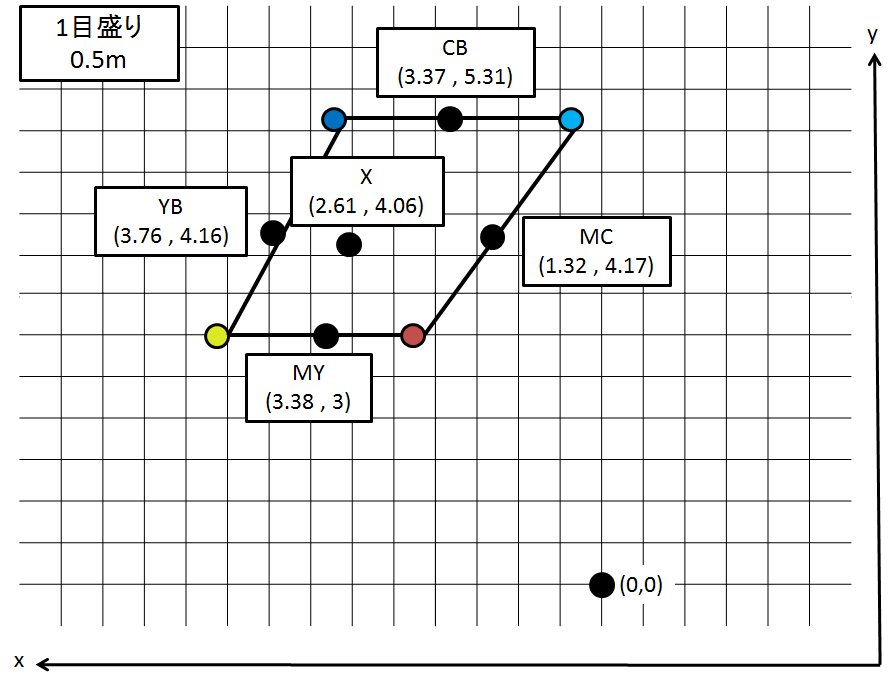
\includegraphics[clip,width=1.05\hsize]{img/ongenichi.png}
  \caption{音源位置}\label{fig:ongenichi}
\end{figure}




%\section{音圧校正手法の有効性}
%\section{クロックずれ校正手法の有効性}
%\section{隣接ノードでない端末間の各種手法の有効性}


\section{barker coded chirpについて}
以前使用していたbarker coded chirpによるパルスを利用した端末間距離測定の評価も行った.
MacBookAir13インチ3台を,1辺2mの正三角形に配置し,
先述のアルゴリズムにより各端末間距離を10回計測した.
表\ref{tab:estdistance}に,計測された各端末間の信号伝達時間と,その伝達時間から音速を340m/sと仮定したときの計測距離をそれぞれ示す.
最頻値はカーネル密度推定により求めた.

\begin{table}[p]\centering
  \caption{端末間距離計測結果}
  \label{tab:estdistance}
  \begin{tabular}{l|rrrrr}
    \hline
    端末間&平均(s)&最頻値(s)&中央値(s)&標準偏差&計測距離(m)\\
    \hline
    A-B&0.0061&0.0061&0.0061&0.00001&2.08\\
    A-C&0.0066&0.0067&0.0067&0.00013&2.27\\
    B-C&0.0057&0.0057&0.0057&0.00001&1.94\\
    \hline
  \end{tabular}
\end{table}


その結果,最大27cm(A-C間),最小6cm(B-C)の誤差にとどまった.
MacBookAir13インチの幅は30cm程度あるため,推定距離の誤差を考慮しても高精度に測距・同期できたと言える.
また,標準偏差も極めて低く,高確度に測定できていることが分かる.
この同期・測距の後,被験者1名に対して音源を各端末とも同一のボリュームで再生したところ,同一の音源として聴こえ,端末の三角形の内部に音像が定位された.
また,三角形の一辺が大きいと,受聴者がその三角形の外側の時には,みかけ音源の幅(ASW: auditory source width)が大きくなり,受聴者が三角形の内側の時に音に包まれた感じ(LEV: listener envelopment)を体験した.
